%========================================================
% EXPERIMENT 2 — Source--Fiber Operating Region
%                under Single-Arm PMD
%========================================================

\subsection{Objective and Numerical Setup}

The second numerical experiment introduces the frequency-dependent PMD model and
investigates how the source spectral bandwidth and the fiber differential group
delay jointly determine the BBM92 operating region.

A single-arm configuration is considered in order to isolate this dependence.
The photon propagating through arm \(A\) experiences first-order PMD with a fixed
birefringence axis, while arm \(B\) is kept ideal. The polarization
transformation at the carrier frequency is assumed to be compensated, so that
only the frequency-dependent PMD contribution is retained.

The input polarization state is the reference Bell state \( |\Psi^+\rangle \).
A Gaussian spectral distribution is used, with spectral bandwidth
\(\sigma_\omega\) varied over

\begin{equation}
2.5\times10^{10}
\leq
\sigma_\omega
\leq
2.0\times10^{11}
\;\mathrm{rad/s},
\end{equation}

while the differential group delay is varied over

\begin{equation}
0
\leq
\Delta\tau
\leq
30
\;\mathrm{ps}.
\end{equation}

The numerical spectral integration uses \(81\) frequency nodes per arm over a
window of \(\pm6\sigma_\omega\). The PMD axis in arm \(A\) is chosen along the
\(x\)-axis of the Bloch sphere. With this orientation, the diagonal-basis
correlation is protected, while the computational-basis correlation is degraded
by the frequency-dependent propagation.

For every pair \((\sigma_\omega,\Delta\tau)\), the frequency-resolved
polarization state is propagated and the unresolved spectral degree of freedom
is traced out according to
Eq.~\eqref{eq:pmd_two_arm_reduced_polarization_state}. The resulting polarization
state is characterized through concurrence and the two BBM92 error rates
\(Q_Z\) and \(Q_X\).

The operational classification is based on the worst-basis error

\begin{equation}
Q_{\mathrm{worst}}
=
\max(Q_Z,Q_X),
\label{eq:exp2_worst_basis_qber}
\end{equation}

with the adopted threshold

\begin{equation}
Q_{\mathrm{worst}}
<
Q_{\mathrm{th}},
\qquad
Q_{\mathrm{th}}=0.11.
\label{eq:exp2_operational_condition}
\end{equation}


%--------------------------------------------------------
% Source--Fiber BBM92 Operating Region
%--------------------------------------------------------

\subsection{Source--Fiber BBM92 Operating Region}

Figure~\ref{fig:exp2_single_arm_pmd_operating_region} shows the worst-basis QBER
over the source--fiber parameter space.

\begin{figure}[htbp]
    \centering

    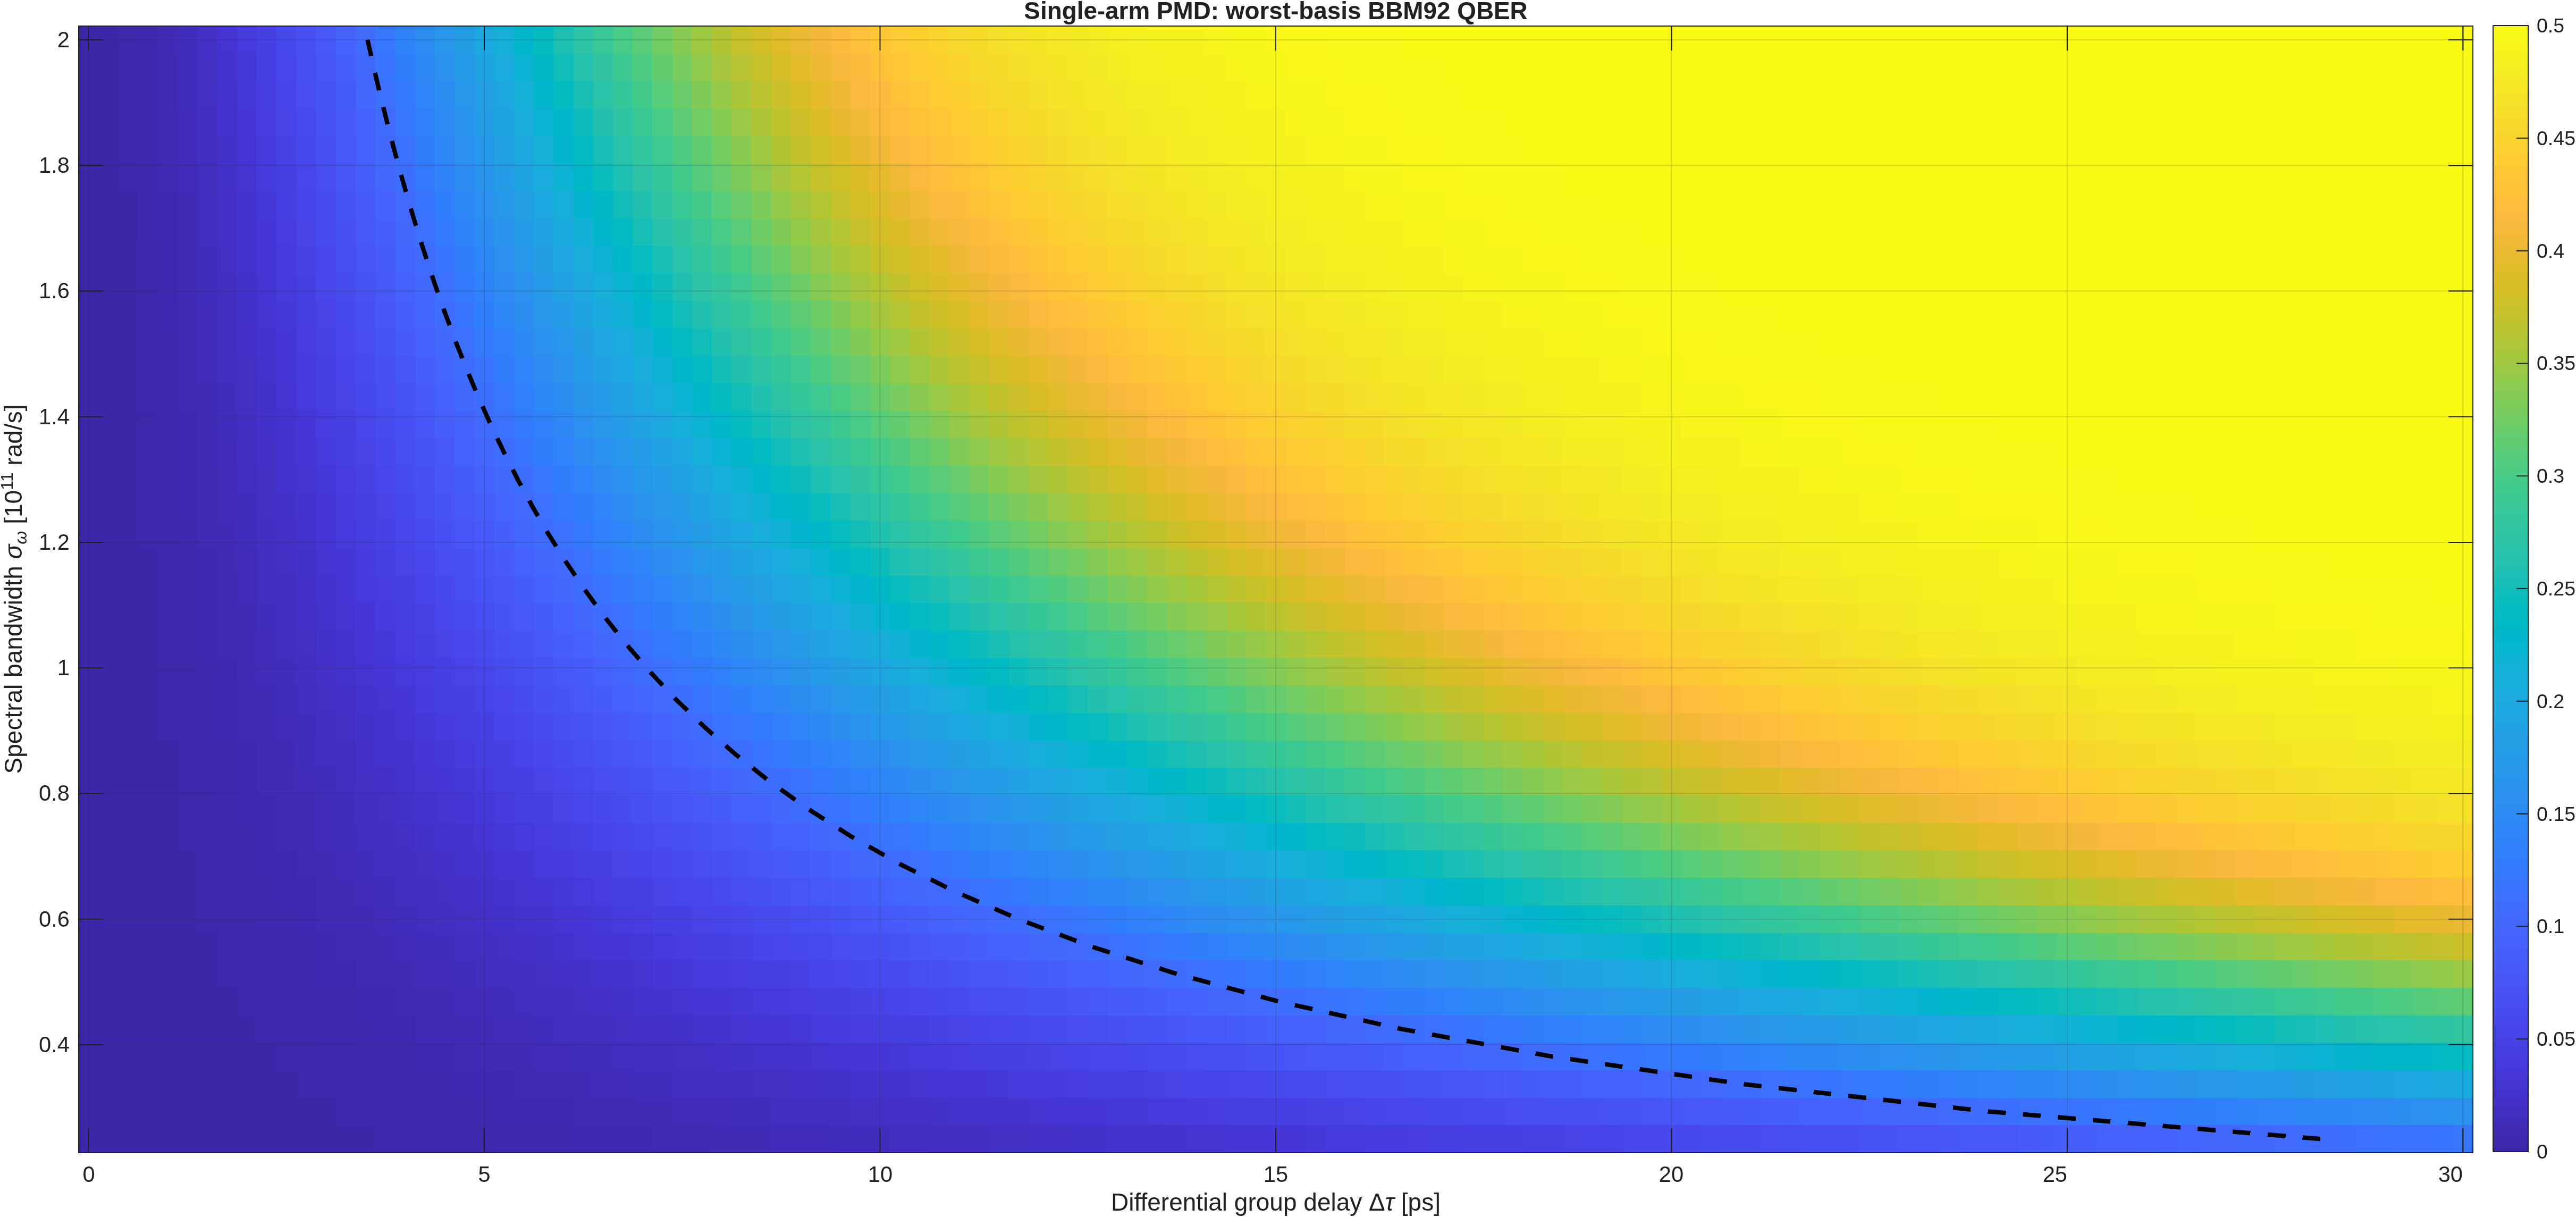
\includegraphics[
        width=0.95\textwidth
    ]{
        figures/experiment_2/single_arm_pmd_operating_region.png
    }

    \caption{
        Worst-basis BBM92 QBER for single-arm first-order PMD as a function of
        the photon spectral bandwidth \(\sigma_\omega\) and the differential
        group delay \(\Delta\tau\). The dashed curve identifies the adopted
        BBM92 operating boundary \(Q_{\mathrm{worst}}=Q_{\mathrm{th}}\), with
        \(Q_{\mathrm{th}}=0.11\).
    }

    \label{fig:exp2_single_arm_pmd_operating_region}
\end{figure}

The operating region lies below and to the left of the dashed boundary. For a
fixed spectral bandwidth, increasing the DGD increases the frequency dependence
of the polarization transformation and consequently the QBER. Conversely, for a
fixed DGD, a broader photon spectrum samples a larger range of
frequency-dependent polarization transformations and therefore produces the same
effect.

The boundary consequently exhibits an approximately inverse dependence between
the maximum tolerable DGD and the source bandwidth. This behavior follows
directly from the normalized PMD parameter introduced in
Eq.~\eqref{eq:normalized_pmd_parameter},

\begin{equation}
\chi
=
\sigma_\omega |\Delta\tau|.
\label{eq:exp2_normalized_pmd_parameter}
\end{equation}

For the Gaussian spectrum considered here, Chapter~\ref{ch:02_fiber_channel_modeling}
showed that the surviving polarization coherence is

\begin{equation}
|\kappa|
=
e^{-\chi^2/2},
\end{equation}

as given by Eq.~\eqref{eq:gaussian_pmd_coherence_normalized}. The numerical
operating boundary is therefore expected to correspond to an approximately
constant value of \(\chi\), rather than to an independent limitation on
\(\sigma_\omega\) or \(\Delta\tau\).


%--------------------------------------------------------
% Entanglement at the Operational Boundary
%--------------------------------------------------------

\subsection{Entanglement at the Operational Boundary}

The corresponding concurrence is shown in
Fig.~\ref{fig:exp2_single_arm_pmd_concurrence}. The same BBM92 operating boundary
is superimposed on the state-quality map.

\begin{figure}[htbp]
    \centering

    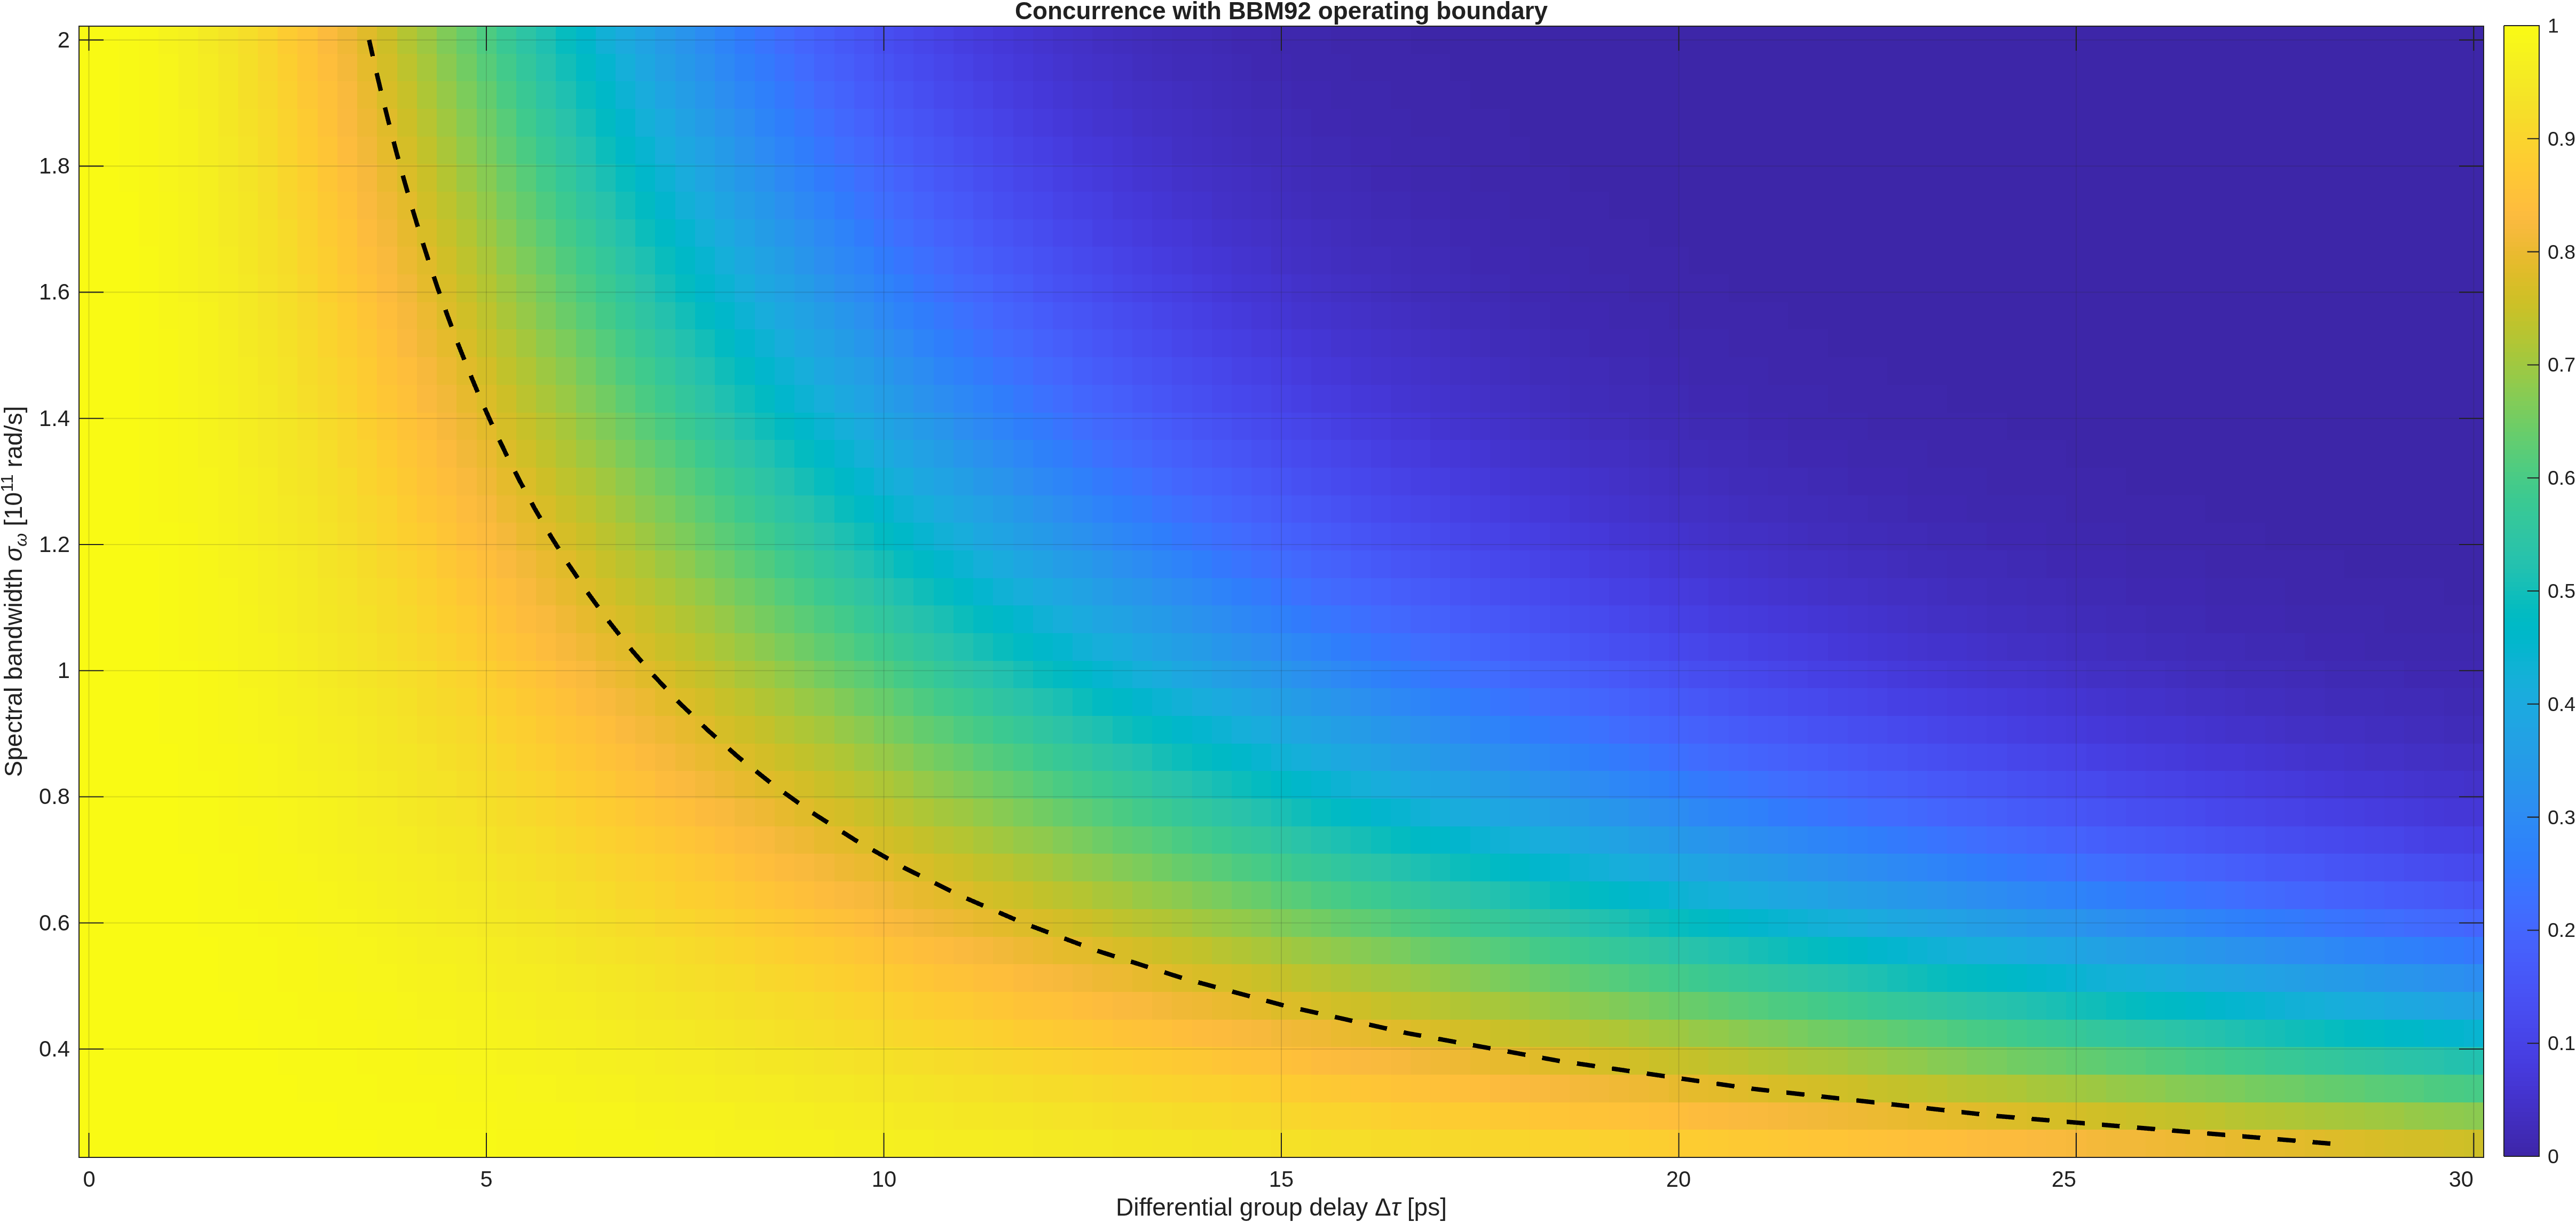
\includegraphics[
        width=0.95\textwidth
    ]{
        figures/experiment_2/single_arm_pmd_concurrence_map.png
    }

    \caption{
        Concurrence of the reduced polarization state under single-arm
        first-order PMD. The dashed curve is the BBM92 operating boundary
        obtained from \(Q_{\mathrm{worst}}=0.11\), rather than from an imposed
        concurrence threshold.
    }

    \label{fig:exp2_single_arm_pmd_concurrence}
\end{figure}

The concurrence decreases continuously as the product
\(\sigma_\omega|\Delta\tau|\) increases. This behavior is consistent with the
analytical single-arm Gaussian result derived in
Eq.~\eqref{eq:single_arm_pmd_concurrence_analytical},

\begin{equation}
C(\chi)
=
e^{-\chi^2/2}.
\end{equation}

Importantly, the dashed curve in
Fig.~\ref{fig:exp2_single_arm_pmd_concurrence} is not defined by selecting an
independent minimum acceptable concurrence. It is obtained exclusively from the
BBM92 QBER requirement and subsequently represented on the concurrence map.
The figure therefore shows the amount of entanglement remaining when the
operational QBER boundary is reached.


%--------------------------------------------------------
% Numerical and Analytical Boundary
%--------------------------------------------------------

\subsection{Operating-Boundary Analysis}

The numerical results confirm that the source bandwidth and fiber DGD enter the
operational boundary predominantly through the normalized PMD parameter
\(\chi=\sigma_\omega|\Delta\tau|\).

For the adopted QBER threshold, the analytical single-arm Gaussian model gives

\begin{equation}
\chi_{\mathrm{th}}^{\mathrm{ana}}
=
0.704927.
\label{eq:exp2_analytical_chi_threshold}
\end{equation}

The numerical parameter sweep gives

\begin{equation}
\overline{\chi}_{\mathrm{th}}^{\mathrm{num}}
=
0.704872,
\qquad
\sigma_{\chi_{\mathrm{th}}}
=
5.505\times10^{-5},
\label{eq:exp2_numerical_chi_threshold}
\end{equation}

with a maximum absolute deviation from the analytical boundary of

\begin{equation}
\max
\left|
\chi_{\mathrm{th}}^{\mathrm{num}}
-
\chi_{\mathrm{th}}^{\mathrm{ana}}
\right|
=
2.044\times10^{-4}.
\label{eq:exp2_chi_boundary_error}
\end{equation}

The concurrence evaluated along the numerical BBM92 boundary is correspondingly

\begin{equation}
\overline{C}_{\mathrm{th}}
=
0.780000,
\end{equation}

with a standard deviation of only \(1.902\times10^{-9}\) over the explored
bandwidth range. The approximately constant concurrence along the boundary is a
consequence of the single-parameter dependence of this particular fixed-axis
Gaussian PMD model and should therefore not be interpreted as a universal
concurrence threshold for BBM92 operation.

The simulation also reproduces the expected limiting behavior at zero DGD:
the propagated state remains the original Bell state, with unit concurrence and
zero QBER in both measurement bases. For the selected \(x\)-oriented PMD axis,
the diagonal basis remains protected throughout the sweep,
\(Q_X=0\), while \(Q_Z\) determines the operating boundary.

The experiment therefore reduces the two-dimensional source--fiber parameter
space to a physically meaningful normalized condition,

\begin{equation}
\boxed{
\sigma_\omega|\Delta\tau|
<
\chi_{\mathrm{th}}
\simeq
0.705,
}
\label{eq:exp2_final_operational_condition}
\end{equation}

for the specific single-arm, fixed-axis, Gaussian PMD configuration considered
here. This result provides the first direct source--fiber operating map of the
numerical analysis and establishes the reference case for the two-arm and
spectrally correlated configurations considered in the following experiment.